\documentclass[10pt]{ctexart}
\usepackage{amsmath,amsfonts,amssymb,amsthm}
\usepackage[a4paper,left=2.5cm,right=2.5cm,top=2cm,bottom=2cm]{geometry}
\usepackage{graphicx,booktabs}
\usepackage{float,bm}
\usepackage{subfigure}
\author{2000012425 张弛}
\title{计算物理第五次作业}
\CTEXsetup[format={\Large\bfseries}]{section}
\newtheorem*{answer}{答}
\newtheorem*{solution}{解}
\newtheorem*{fuck}{证明}
\begin{document}
\maketitle
1.参考课件《偏微分方程A》,对Kruskal,Zalusky孤立子问题,给出数值解(随时间演化的动画示意图,或者代表性时刻的帧图)及
说明,注意保证大$t$时数值结果的稳定性。
$$
\begin{cases}
    u_t+uu_x+\delta^2u_{xxx}=0,\\
    u(x,0)=\cos{(\pi x)}, & 0\leq x \leq 2.
\end{cases}$$
$u,u_x,u_{xx}$为在$[0,2]$上的周期函数。
\begin{solution}
一些差分
$$\frac{\partial u}{\partial t}=\frac{u_{i,j+1}-u_{i,j}}{\Delta t},\frac{\partial u}{\partial x}=\frac{u_{i+1,j}-u_{i-1,j}}{2\Delta x}.$$
然后一点平均方法
$$u=\frac{u_{i-1,j}+u_{i,j}+u_{i+1,j}}{3}.$$
得到差分公式
$$u_{i,j+1}=u_{i,j}-\frac{\Delta t}{\Delta x}\left[\frac{1}{6}(u_{i+1,j}-u_{i-1,j})(u_{i-1,j}+u_{i,j}+u_{i+1,j})+\frac{\delta^2}{2(\Delta x)^2}(u_{i+2,j}+2u_{i-1,j}-2u_{i+1,j}-u_{i-2,j})\right].$$
近似一下变量$t$为中心差分情形的Von Neumann稳定条件
$$\frac{1}{(\Delta x/\Delta t)}\left[|u|+4\left(\frac{\delta}{\Delta x}\right)^2\right]\leq 1.$$
一些变量步数和步长的选取
$$0\leq x\leq 2,\Delta x=2/128,$$
$$0\leq t \leq 12.6,\Delta t=12.6/600000.$$
然后取$\delta=0.022$.借助程序"HW5计物第一题.py"得到动图"KZ.gif"。

可以看到随着时间演进,余弦波开始挤压产生截波。然后色散项$u_{xxx}$开始起作用,解变成一列由8个类$sech$函数组成的波,速度快的波会追上慢的波,吞入然后又吐出。经过一段时间,原先的余弦波又出现了。
不过这时稳定性已经不佳了。
\end{solution}
2.参考课件《偏微分方程B》,使用谱方法或者其他方法求解2维扩散方程,给出数值解(随时间演化的动画示意图,或者代表性时刻的帧图)及说明:
$$\frac{\partial T}{\partial t}=D\frac{\partial^2 T}{(\partial x)^2}+D\frac{\partial^2 T}{(\partial y)^2}.$$
其中$D=1,0\leq x\leq 1,0\leq y\leq 1,$\\
\noindent $x$方向的边界条件为$T(x=0,y)=T(x=1,y)=0,$\\
\noindent $y$方向的边界条件为$dT/dy(x,y=0)=dT/dy(x,y=1)=0.$
\begin{solution}
    使用谱方法。$x$方向为Dirichlet边界条件,将解按照$x$进行傅里叶展开
    $$T(x,y,t)=\sum\limits_{i=1}^{\infty}\hat{T}_{i}(y,t)\sin{(i\pi x)}.$$
    一些差分
    $$t_n=t_0+n\delta t,x_i=x_0+i\delta x,y_j=y_0+j\delta y.$$
    其中$0\leq i\leq I,0\leq j \leq J.$差分化后的傅里叶展开的截断形式
    $$T_{i,j}^{n}=\sum\limits_{k=0}^{I}\hat{T}_{k,j}^{n}\sin{(ik\pi/I)}.$$
    原方程差分化,使用了Crank-Nicholson方法,其中$y$变量中心差分
    $$\frac{T_{i,j}^{n+1}-T_{i,j}^{n}}{\delta t}=\frac{D}{2}\left[\left(\frac{\partial^2T}{\delta x^2}\right)_{i,j}^{n+1}+\left(\frac{\partial^2T}{\delta x^2}\right)_{i,j}^{n}\right]+\frac{D}{2}\left[\frac{T_{i,j-1}^{n+1}-2T_{i,j}^{n+1}+T_{i,j+1}^{n+1}}{(\delta y)^2}+\frac{T_{i,j-1}^{n}-2T_{i,j}^{n}+T_{i,j+1}^{n}}{(\delta y)^2}\right].$$
    则差分过后的傅里叶分量满足的方程
    $$-\frac{C}{2}\hat{T}_{i,j-1}^{n+1}+\{1+C(1+i^2\kappa^2/2)\}\hat{T}_{i,j}^{n+1}-\frac{C}{2}\hat{T}_{i,j+1}^{n+1}=\frac{C}{2}\hat{T}_{i,j-1}^{n}+\{1-C(1+i^2\kappa^2/2)\}\hat{T}_{i,j}^{n}+\frac{C}{2}\hat{T}_{i,j+1}^{n}.$$
    其中$C=D\frac{\delta t}{(\delta y)^2},\kappa=\pi\delta y.$边界条件比较简单
    $$\hat{T}_{i,0}^{n}=\hat{T}_{i,1}^{n},\hat{T}_{i,J-1}^{n}=\hat{T}_{i,J}^{n}.$$
    是个三对角矩阵。取定一些差分的格子
    $$I=J=128,\delta t=0.0001.$$
    初始条件为
    $$T(x,y,0)=\eta(0.1-|x-0.5|)\eta(0.1-|y-0.5|).$$
    需要用到差分形式的傅里叶变换
    $$\hat{T}_{i,j}^{n}=\frac{2}{I}\sum\limits_{k=0}^{I}T_{k,j}^{n}\sin{(ik\pi/I).}$$
    时间范围
    $$0\leq t \leq 0.1,N=1000.$$
    用Thomas算法来解三对角线性方程。借助程序"HW5计物第二题.py"得到动图"Heat.gif"。

    可以看到随着时间演进,中心方块的浓度开始扩散,近似为圆形,逐渐扩大,由于边界条件的限制,在时间充分大后,
    会形成边界平行于$y$轴的等浓度层。
\end{solution}
3.考虑由一下初始条件和边界条件给出的振动方膜的二维波动方程:
$$
\begin{cases}
    \lambda\left(\frac{\partial^2 u}{\partial x^2}+\frac{\partial^2 u}{\partial t^2}\right)=\frac{\partial^2 u}{\partial t^2}, & x,y\in[0,1],t\geq 0,\\
    u(x,y,0)=\sin{(\pi x)}\sin{(2\pi y)}, & x,y\in{(0,1)},\\
    u=0\ boundary, & t\geq 0,\\
    {\partial u}/{\partial t}|_{t=0}, & x,y\in(0,1).
\end{cases}$$
边界由$x=0,x=1,y=0$及$y=1$给定。$\lambda$可以取为1.

1)使用分离变量法给出该方程的解析解。
\begin{solution}
    直接将解按照本征函数展开
    $$u(x,y,t)=\sum\limits_{mn}c_{mn}(t)\sin{(m\pi x)}\sin{(n\pi y)}.$$
    代入原方程,得
    $$\ddot{c}_{mn}(t)+(m^2+n^2)\pi^2c_{mn}=0.$$
    知道初始条件
    $$\begin{cases}
        c_{mn}(0)=\delta_{m1}\delta_{n2},\\
        \dot{c}_{mn}(0)=0.
    \end{cases}$$
    解得
    $$c_{mn}(t)=\delta_{m1}\delta_{n2}\cos{(\sqrt{5}\pi t)}.$$
    则解析解为
    $$u(x,y,t)=\sin{(\pi x)}\sin{(2\pi y)}\cos{(\sqrt{5}\pi t)}.$$
\end{solution}
2)使用二维差分网格,写出求解该方程的显式方法的算法,并编写数值求解离散波动方程的程序。特别是描述如何处理边界条件和初始条件,
并将结果与封闭形式的解决方案进行比较。
\begin{solution}
    使用谱方法。$x$方向为Dirichlet边界条件,将解按照$x$进行傅里叶展开
    $$u(x,y,t)=\sum\limits_{i=1}^{\infty}\hat{u}_{i}(y,t)\sin{(i\pi x)}.$$
    一些差分
    $$t_n=t_0+n\delta t,x_i=x_0+i\delta x,y_j=y_0+j\delta y.$$
    其中$0\leq i\leq I,0\leq j \leq J.$差分化后的傅里叶展开的截断形式
    $$u_{i,j}^{n}=\sum\limits_{k=0}^{I}\hat{u}_{k,j}^{n}\sin{(ik\pi/I)}.$$
    原方程差分化,使用了Crank-Nicholson方法,其中$y$变量和$t$变量使用中心差分
    $$\frac{u_{i,j}^{n+1}-2u_{i,j}^{n}+u_{i,j}^{n-1}}{(\delta t)^2}=\frac{\lambda}{2}\left[\left(\frac{\partial^2u}{\delta x^2}\right)_{i,j}^{n+1}+\left(\frac{\partial^2u}{\delta x^2}\right)_{i,j}^{n}\right]+\frac{\lambda}{2}\left[\frac{u_{i,j-1}^{n+1}-2u_{i,j}^{n+1}+u_{i,j+1}^{n+1}}{(\delta y)^2}+\frac{u_{i,j-1}^{n}-2u_{i,j}^{n}+u_{i,j+1}^{n}}{(\delta y)^2}\right].$$
    则差分过后的傅里叶分量满足的方程
    $$-\frac{C}{2}\hat{u}_{i,j-1}^{n+1}+\{1+C(1+i^2\kappa^2/2)\}\hat{u}_{i,j}^{n+1}-\frac{C}{2}\hat{u}_{i,j+1}^{n+1}=\frac{C}{2}\hat{u}_{i,j-1}^{n}+\{2-C(1+i^2\kappa^2/2)\}\hat{u}_{i,j}^{n}+\frac{C}{2}\hat{u}_{i,j+1}^{n}-\hat{u}_{i,j}^{n-1}.$$
    其中$C=\lambda\left(\frac{\delta t}{\delta y}\right)^2,\kappa=\pi\delta y.$边界条件比较简单
    $$\hat{u}_{i,0}^{n}=0,\hat{u}_{i,J}^{n}=0.$$
    初值条件直接离散傅里叶变换即可
    $$\hat{u}_{i,j}^{0}=\frac{2}{I}\sum\limits_{k=0}^{I}u_{k,j}^{0}\sin{(ik\pi/I).}$$
    一阶初值条件写为
    $$\hat{u}_{i,j}^{1}=\hat{u}_{i,j}^{0}.$$
    取定一些差分的格子
    $$I=J=128,\delta t=0.001.$$
    时间范围
    $$0\leq t \leq 1,N=1000.$$
    借助程序"HW5计物第三题数值法.py"得到动图"OscillationNum.gif"。

    另外借助程序"HW5计物第三题解析法.py"得到动图"OscillationAna.gif"。

    可以看到两种方法得到的结果看不出差别。都是标准的本征振动形式,且频率振幅相同。
\end{solution}
3)给出不同差分步长($\Delta t,\Delta x$及$\Delta y$)情形的数值表现,特别是考虑和校验数值稳定性条件(此处可以设置$\lambda=1,2$等不同值):
$$\Delta t\leq \frac{1}{\sqrt{\lambda}}\left(\frac{1}{\Delta x^2}+\frac{1}{\Delta y^2}\right)^{-1/2}.$$
\begin{solution}
    上一题已经给出一种较稳定的情况,下面看两个另外的情况。

    取
    $$\Delta t=0.1,\Delta x=1/128,\Delta y=1/128.$$
    此时
    $$\Delta t\sqrt{\frac{1}{\Delta x^2}+\frac{1}{\Delta y^2}}=18\geq 1.$$
    借助程序"HW5计物第三题稳定性比较.py"得到动图"OscillationTlarge.gif"。发现振动发生了不应该发生的衰减。

    取
    $$\Delta t=0.001,\Delta x=1/128,\Delta y=1/16.$$
    此时
    $$\Delta t\sqrt{\frac{1}{\Delta x^2}+\frac{1}{\Delta y^2}}=0.13\leq 1.$$
    借助程序"HW计物第三题稳定性比较.py"得到动图"OscillationLattice.gif"。由于满足稳定性,振动模式保持正确,但是由于差分格子较大,出现锐利边缘。
\end{solution}
4)对$\Delta x=\Delta y$情形,给出结果的动画展示。
\begin{answer}
    比如前面的"OscillationNum.gif"和"OscillationTlarge.gif"。
\end{answer}
4.参考课件《随机数及简明概率论》,选取某种程序自带的随机数产生方法,产生一组$[0-1]$之间均匀分布的随机数,统计$[0-0.1-0.2...0.9-1.0]$各个区间的撒点数。
重复上述步骤多次(如:10000次)

1)请数值模拟,得到落入区间如$[0.3-0.4]$内的随机数的比例,给出这个比例的$10000$次数值的分布曲线,并给予论述说明;
\begin{solution}
    使用python的random函数,每次模拟产生1000个随机数,然后统计相关比例并画出比例曲线。

    借助程序"HW5计物第四题随机性统计.py"得到下图
    \begin{figure}[H]
        \centering
        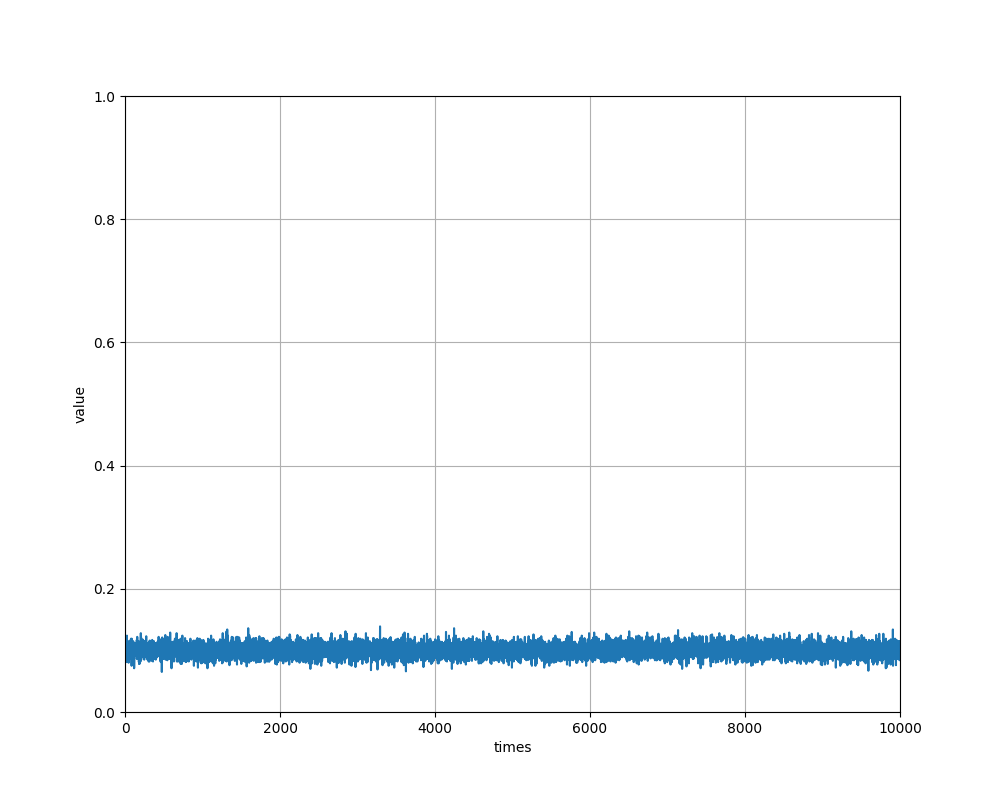
\includegraphics[width=10cm]{prob.png}
        \caption{random函数随机性统计}
    \end{figure}
    当然我感觉散点图更好
    \begin{figure}[H]
        \centering
        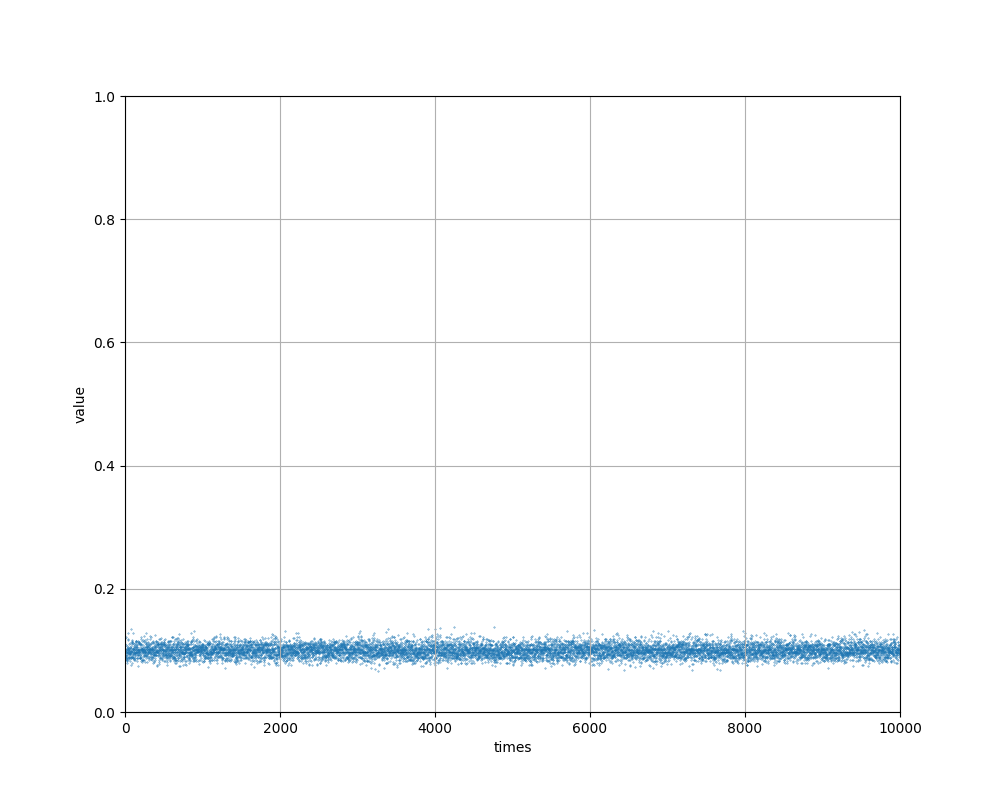
\includegraphics[width=10cm]{prob1.png}
        \caption{random函数随机性统计}
    \end{figure}
    可以看出来比例基本在$0.1$上下波动,比较稳定均匀。
\end{solution}
2)参照课件,构建Chi2检验随机数的性质,并论述结果。
\begin{solution}
    列联表检验。生成$20000$个随机数,交替分成两组,第一组作为$10000$个$x$,第二组作为$10000$个$y$,共$10000$个点。这$10000$个点应当随机分布。
    考虑$x-y$平面,划分为$10\times 10$的格子,统计这$10000$个点落入每个方格的频次$n_{ij}$,将理论频次$m_{ij}=100$作为平均值,算出
    统计检验量
    $$\chi^2=\sum\limits_{i,j=1}^{k}\frac{(n_{ij}-m_{ij})^2}{m_{ij}}.$$
    卡方检验自由度
    $$n=9999.$$
    由程序"HW5计物第四题卡方独立性检验.py"得到假设"random函数产生随机数是独立的"的置信概率为100\%,十次模拟结果都是100\%。
\end{solution}
\end{document}